\synctex=0
\documentclass[tikz]{standalone}
\usetikzlibrary{arrows.meta, positioning}
\usetikzlibrary{ decorations.pathmorphing, decorations.pathreplacing, decorations.shapes}
\definecolor{dodgerblue}{HTML}{1E90FF}
\definecolor{gray}{HTML}{708090}


\newcommand{\DrawComplexity}{
    \clip (-1.5,-1.5) rectangle (1.5,1.5);

        % Fixamos a semente para manter o mesmo padrão gerado toda vez
        \pgfmathsetseed{314}

        % Varredura numa grade fina (que será "bagunçada" depois)
        \foreach \x in {-26,...,26} {
            \foreach \y in {-26,...,26} {
                % Posição base na grade (espaçamento de 0.06)
                \pgfmathsetmacro{\px}{\x*0.06}
                \pgfmathsetmacro{\py}{\y*0.06}
                
                % Coordenadas polares (+0.001 para evitar erro de divisão por zero no centro)
                \pgfmathsetmacro{\theta}{atan2(\py+0.001, \px+0.001)}
                \pgfmathsetmacro{\r}{sqrt(\px*\px + \py*\py)}
                
                % --- MATEMÁTICA DO CAOS E COMPLEXIDADE ---
                
                % 1. O estiramento (Advecção): Cria braços espirais
                % 800 é a taxa de torção. Quanto maior, mais enrolada a espiral.
                \pgfmathsetmacro{\spiral}{cos(\theta - 1000*\r)}
                
                % 2. O dobramento (Perturbação): Quebra a espiral em ilhas e filamentos
                \pgfmathsetmacro{\perturb}{0.5*sin(500*\px)*cos(500*\py)}
                
                % 3. A memória do estado inicial: Mantém o centro mais concentrado (círculo)
                \pgfmathsetmacro{\cboost}{\r < 1.5 ? 2.5*exp(-5*\r*\r) : 0}
                
                % Equação agregada: Ordem (centro+espiral) + Caos (perturbação+ruído)
                \pgfmathsetmacro{\val}{\spiral + \perturb + 0.8*rand + \cboost}
                
                % Limiar da transição: se o valor for maior que 0.4, existe corante ali
                \pgfmathparse{\val > 0.4 ? 1 : 0}
                \ifnum\pgfmathresult=1
                    % Adiciona um "jitter" (tremor) para destruir o padrão de grade perfeito
                    \pgfmathsetmacro{\jx}{\px + 0.025*rand}
                    \pgfmathsetmacro{\jy}{\py + 0.025*rand}
                    
                    % Varia o raio da bolinha para dar um aspecto orgânico de gotículas
                    \pgfmathsetmacro{\rad}{0.03 + 0.05*abs(rand)}
                    
                    \fill[dodgerblue,opacity=rnd] (\jx, \jy) circle (\rad);
                \fi
            }
        }
}

\begin{document}

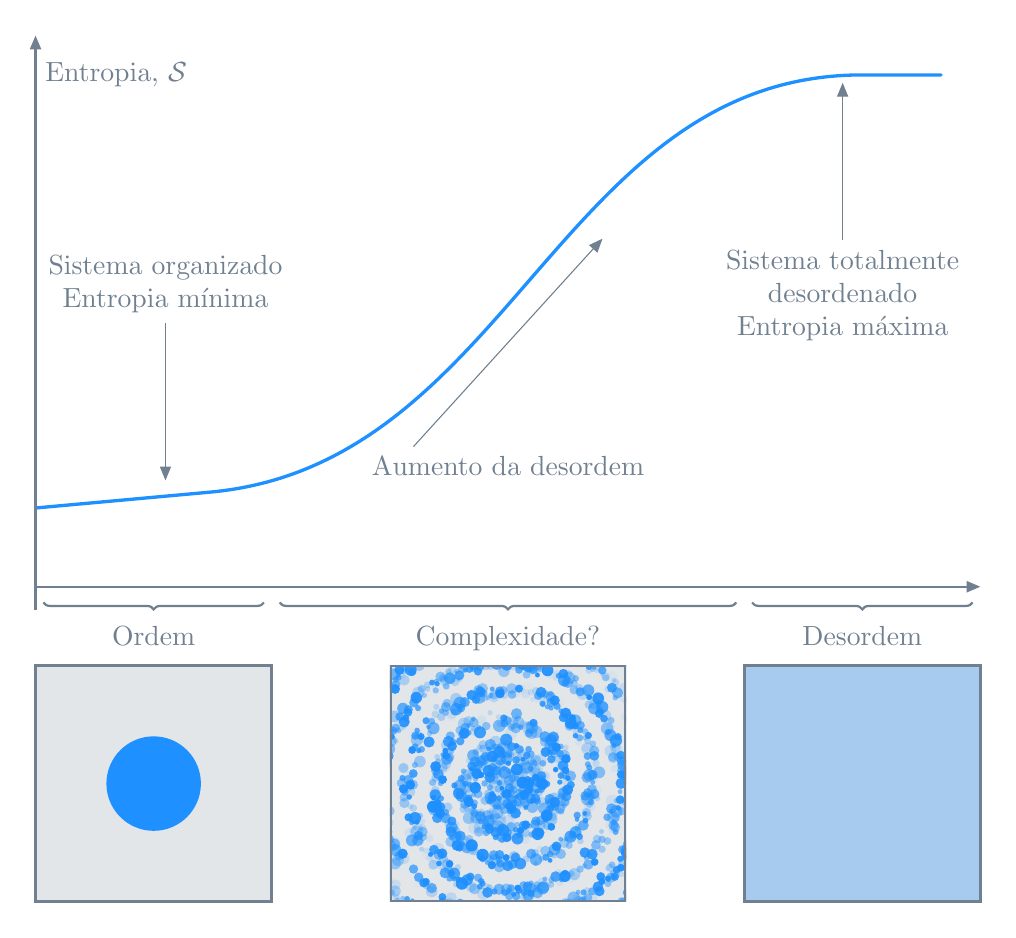
\begin{tikzpicture}
    \useasboundingbox (-0.1,-4.1) rectangle (12.1,7.1);
    \coordinate(S0) at (0,1);
    \coordinate(S1) at (2.2,1.2);
    \coordinate(S2) at (10.5,6.5);
    \coordinate(S3) at (11.5,6.5);

    \draw[dodgerblue,very thick,line cap=round,line join=round]
        (S0)
            --
        (S1)
            to[out=5, in=180]
        (S2)
            --
        (S3);


    \draw[-{Triangle[length=0.5em, width=0.4em]}, gray] (1.65,3.35) -- (1.65,1.35);
    \node[anchor=south,align=center, gray] at (1.65,3.35) {Sistema organizado\\ Entropia mínima};
    
    \draw[-{Triangle[length=0.5em, width=0.4em]}, gray] (10.25,4.4) -- (10.25,6.4);
    \node[anchor=north,align=center, gray] at (10.25,4.4) {Sistema totalmente\\ desordenado\\Entropia máxima};
    
    \draw[-{Triangle[length=0.5em, width=0.4em]}, gray] (4.8,1.1*4.8-3.5) -- (7.2,1.1*7.2-3.5);
    \node[gray,anchor=north] at (6,1.1*4.8-3.5) {Aumento da desordem};

    \draw[-{Triangle[length=0.5em, width=0.4em]}, thick, gray] (0,-0.3) -- (0,7);
    \draw[-{Triangle[length=0.5em, width=0.4em]}, thick, gray] (0,0) -- (12,0);
    \node[anchor=west, gray] at (0,6.5) {Entropia, $\mathcal{S}$};
    
    \draw[decorate,decoration=brace, thick,gray]
        (3-0.1,-0.2) -- (0.1,-0.2) node[midway,anchor=north,yshift=-0.5em,align=center] {Ordem};
    \begin{scope}[shift={(1.5,-2.5)}]
        \fill[gray,opacity=0.2] (-1.5,-1.5) rectangle (1.5,1.5);
        \fill[dodgerblue] (0,0) circle (0.6);
        \draw[gray, very thick] (-1.5,-1.5) rectangle (1.5,1.5);
    \end{scope}
    
    \draw[decorate,decoration=brace, thick,gray]
        (9-0.1,-0.2) -- (3+0.1,-0.2) node[midway,anchor=north,yshift=-0.5em,align=center] {Complexidade?};
    \begin{scope}[shift={(6,-2.5)}]
        % Fundo da caixa
        \fill[gray,opacity=0.2] (-1.5,-1.5) rectangle (1.5,1.5);
        
        % Adicionamos um clip para que nenhuma bolinha vaze da caixa
        \DrawComplexity

        % Borda da caixa desenhada por cima no final
        \draw[gray, very thick] (-1.5,-1.5) rectangle (1.5,1.5);
    \end{scope}
        
    \draw[decorate,decoration=brace, thick,gray]
        (12-0.1,-0.2) -- (9+0.1,-0.2) node[midway,anchor=north,yshift=-0.5em,align=center] {Desordem};
    \begin{scope}[shift={(10.5,-2.5)}]
        \fill[gray,opacity=0.2] (-1.5,-1.5) rectangle (1.5,1.5);
        \fill[dodgerblue,opacity=0.3] (-1.5,-1.5) rectangle (1.5,1.5);
        \draw[gray, very thick] (-1.5,-1.5) rectangle (1.5,1.5);
    \end{scope}

    
\end{tikzpicture}

\end{document}